Diferente da figura \ref{module}, o foco da figura \ref{classdiagrama} consiste em apresentar como se dá a estrutura de classes e dos relacionamentos. Ambas situações poderiam ser representadas em uma única figura, contudo o autor decidiu por seccionar em duas, a fim de tornar o processo mais didático. Por esse mesmo motivo não está apresentado neste \textit{UML} todas as classes e propriedades.  

\begin{figure}[H]
  \centering
  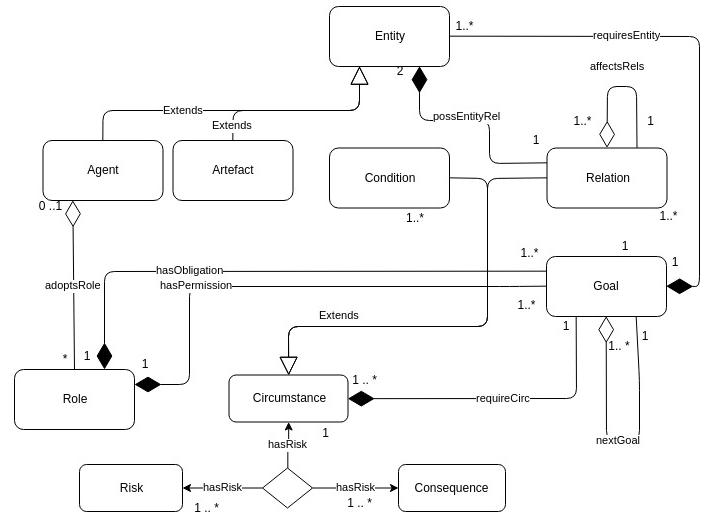
\includegraphics[width=1\linewidth]{figure/Class.jpeg} 
  \caption{Diagrama de classes do Modelo }
  \label{classdiagrama}
\end{figure}

Uma vantagem deste tipo de diagrama em relação a representação por conjuntos, consiste na ocorrência de uma sintaxe específica para tratar dois pontos relevantes dentro do contexto computacional que são: cardinalidade e relações existenciais. Um dos predicados interessantes de serem analisados, neste contexto, é \textit{adoptsRole} que define um relacionamento fracamente agregada entre \textit{Agent} e \textit{Role}. Isso, pois, dentro do escopo deste modelo, um agente pode existir sem ter um papel, portanto este não é um critério necessário para definir aquele. A cardinalidade se justifica tendo como base o fato de que um agente pode ter um ou mais papéis. 

As relações \textit{hasObligation}, \textit{hasPermission} se dão por meio de agregações fortes tendo em vista que não há sentido para um papel $\rho$ existir sem que esteja vinculado a ao menos um objetivo. Como um papel se relaciona com diversos objetivos, os engenheiros adotaram a cardinalidade de $1$ para $1 .. *$.

Em \textit{UML} questão de conjunto-subconjunto entre $Circumstance$ com $Relation$ e com $Condition$ é definida por meio de classes que possuem esses mesmos nomes. No \textit{UML}, as classes $Relation$ e $Condition$ são extensões da classe $Circumstance$. Dado essa situação, é possível representar a relação \textit{hasRisk} que ocorre entre $Circumstance$, $Relation$ e $Risk$ e isso é feito por meio do ternário entre essas classes. 

Um objetivo não pode ser definido sem saber quais são as entidades $Entity$, relações $Relation$ e consequências $Consequence$ necessárias para que tal objetivo seja alcançado. Por isso os predicados $requiresCirc$ e $requiresEntity$ estabelecem composição forte de suas respectivas classes com $Goal$. Como um objetivo pode apontar para diversas instâncias dessas classes, o autor optou - para cada uma das relações - trabalhar com a cardinalidade 
$1 - 1 .. *$.

No modelo proposto $Relation$ deve estar relacionada com duas entidades. Por esse motivo o predicado $possEntityRel$ faz composição forte com $Entity$ e a sua cardinalidade é dada $1 - 2$. 

A classe $Goal$ possui uma relação consigo mesma dada por $nextGoal$. Essa é uma agregação fraca, pois do contrários seria impossível haver uma única instância desta classe. Isso se deve ao fato de que a primeira instância necessitaria de uma instância de $Goal$ para existir. Contudo, como não há um elemento de $Goal$ antes do primeiro elemento de $Goal$, logo esse primeiro elemento não pode existir. Um objetivo poder ter como próximo um ou mais objetivos, justificando a ocorrência da cardinalidade $1 .. n$. 

O predicado $affectsRels$, por motivos similares a $nextGoal$ deve ter agregação fraca. Como uma relação pode afetar uma ou mais, a cardinalidade adequada para essa circunstância é dada pro $1$ - $1 ..*$